\documentclass[__main__.tex]{subfiles}

\begin{document}

\qtitle{О}{17}
Когерентные источники света, оптическая разность хода лучей, общая схема наблюдения интерференции, условия минимумов и максимумов интенсивности. Условия наблюдения интерференции.\\ 

\begin{definition}
	Интерференцией называется взаимное увеличение(уменьшение) результирующей амплитуды двух или нескольких волн при их наложении друг на друга.
\end{definition}

\begin{definition}
	Два световых источника, способных создать интерференционную картину называются когерентными.
\end{definition}

\begin{theorem}[Условие когерентности источников]
	Два источника света являются когерентными, если
	\begin{enumerate}
		\item они испускают свет одинаковой частоты;
		\item угол между плоскостями колебаний световых векторов
		\footnote{
			векторов напряженности электрических полей электромагнитных волн.
		}
		достаточно мал.
		\item разность фаз в точке наблюдения изменяется незначительно (менее чем на $\pi$) за время усреднения прибора наблюдения.
	\end{enumerate}
\end{theorem}
\begin{proof}
	Рассмотрим две волны одной частоты $\omega$ (первое условие) со световыми векторами:
	\begin{gather*}
	\vec{E}_1 = \vec{E}_{10}e^{-i(\omega t - \varphi_1)},\qquad
	\vec{E}_2 = \vec{E}_{20}e^{-i(\omega t - \varphi_2)},
	\end{gather*}
	где $\vec{E}_{10}, \vec{E}_{20}$ - амплитуды, $\varphi_1, \varphi_2$ - начальные фазы.
	По принципу суперпозиции найдем световой вектор результирующего колебания:
	$$
	\vec{E} = \left(\vec{E}_{10}e^{i\varphi_1}+\vec{E}_{20}e^{i\varphi_2}\right)e^{-i\omega t} =
	\vec{E}_0 e^{-i \omega t}
	$$
	отыщем интенсивность $I$ как квадрат модуля светового вектора:
	\begin{flalign}
	\llabel{o-02-intense}
	\begin{split}
	E^2 &= \left(\vec{E}_{10}e^{i\varphi_1}+\vec{E}_{20}e^{i\varphi_2}\right)
	\left(\vec{E}_{10}e^{-i\varphi_1}+\vec{E}_{20}e^{-i\varphi_2}\right) =\\
	&= E^2_{10} + E^2_{20} + 2(\vec{E}_{10}, \vec{E}_{20})\cos(\varphi_2 - \varphi_1),
	\end{split}
	\end{flalign}
	
	определим $\angle(\vec{E}_{10},\vec{E}_20) = \alpha$, тогда (\lref{o-02-intense}) примет вид:
	\begin{flalign}
	\llabel{o-02-alpha}
	I = I_1 + I_2 + 2\sqrt{I_1 I_2}\cos(\alpha)\langle\cos(\Delta \varphi)\rangle,
	\end{flalign}
	где $\langle\cos(\Delta \varphi)\rangle$ - разность фаз, усредненная по времени наблюдения прибора
	\footnote{
		время отклика прибора измерения, которое, хоть и достаточно мало (для глаза это $0.1~\text{c.}$), но на порядки больше периода колебаний световой волны ($\sim 10^{-15}~\text{c.}$)
	}
	, $I_1 = E_1^2$, $I_2 = E_2^2$.
	
	Из второго условия положим $\cos(\alpha)\approx 1$, тогда (\lref{o-02-alpha}) примет вид:
	\begin{gather}
	\llabel{o-02-mainint}
	I = I_1 + I_2 + 2\sqrt{I_1 I_2}\langle\cos(\Delta \varphi)\rangle
	\end{gather}
	где $2\sqrt{I_1 I_2}\langle\cos(\Delta \varphi)\rangle$ называется интерференционным членом.
	
	Отсюда явно видно, что максимумы интенсивности будут наблюдаться при $\cos(\Delta \varphi)$ = 1, и при одинаковой интенсивности волн мы получим $4I$.
	Соответственно, минимумы получатся, когда косинус равен нулю. При одинаковой интенсивности волн в этом случае интенсивность тоже ноль.
	
	Заметим, что если разность фаз волн изменяются более чем на $\pi$ за время усреднения, то интерференционный член исчезает, и интерференция не наблюдается, иначе происходят периодические изменения интенсивности, т.е. наблюдается интерференция.
\end{proof}

Тогда из определения фазы волны: $\varphi = \vec{k}\vec{x}$ ($\vec{k}$ - волновой вектор, $\vec{x}$ - радиус-вектор) или вдоль светового луча: $\varphi = kl$, причем $l$ - путь, пройденный в среде, и для разных сред:
$$
\varphi = \sum_{i=1}^{N}k_i l_i = k\sum_{i=1}^{N}n_i l_i = kL,
$$
где $k$ - волновое число в вакууме, $n_i$ - коэффициент преломления среды, $L$ называется оптической длиной пути.
Тогда для двух волн одной частоты с фазами $\varphi_1$ и $\varphi_2$ разность их фаз примет вид:
\begin{gather}
\llabel{o-02-phasediff}
\Delta \varphi = k(L_2 - L_1) = k \Delta =
(k = \frac{2\pi}{\lambda}) =
\frac{2\pi}{\lambda}\Delta,
\end{gather}
где $\Delta$ называется оптической разностью хода. 

\begin{wrapfigure}[14]{R}{0.4\linewidth}
	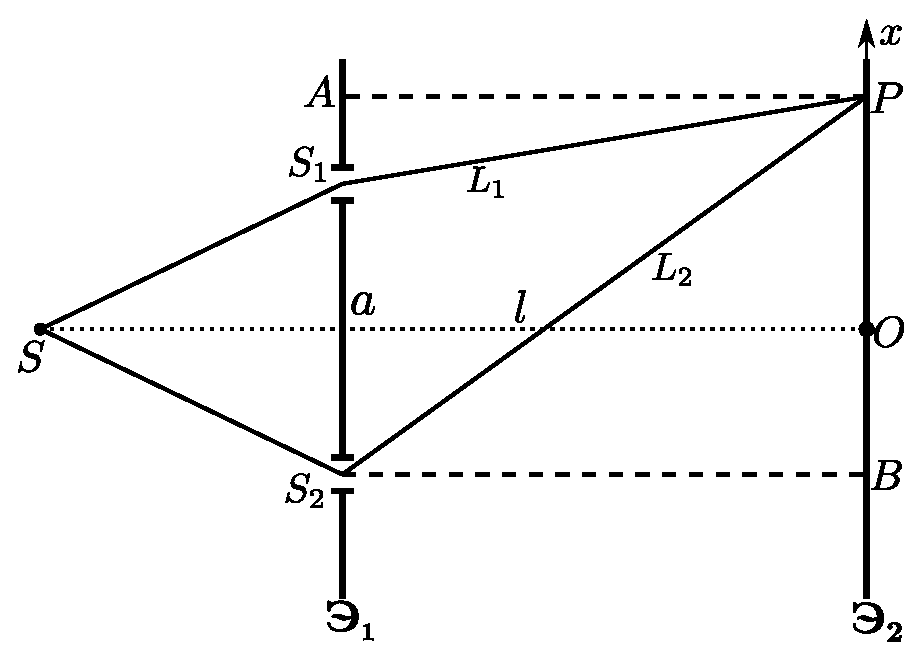
\includegraphics[width=1\linewidth]{img/o-05_1}{}
	\caption{Общая схема наблюдения интерференции}
	\llabel{o-02-scheme}
\end{wrapfigure}

\textit{Условия наблюдения интерференции}\\
Рассмотрим несколько характерных случаев:\\
1. Ортогональность поляризаций волн.
При этом ${{\mathbf  E}}_{{1_{{0}}}}\perp {{\mathbf  E}}_{{2_{{0}}}}$  и   ${{\mathbf  E}}_{{1_{{0}}}}{{\mathbf  E}}_{{2_{{0}}}}=0$. Интерференционные полосы отсутствуют, а контраст равен 0. Далее, без потери общности, можно положить, что поляризации волн одинаковы.\\
2. В случае равенства частот волн ${\mathbf  {}}\Delta \omega = 0$ и контраст полос не зависит от времени экспозиции $V={\frac  {2{{\mathbf  E}}_{{1_{{0}}}}{{\mathbf  E}}_{{2_{{0}}}}}{I_{1}+I_{2}}}.$\\
3. В случае ${\mathbf  {}}\Delta \omega \tau \gg 2\pi$   (радиан) значение функции   ${\displaystyle \mathrm {sin} ({\frac {\Delta \omega \tau }{2}})\simeq 0}$  и интерференционная картина не наблюдается. Контраст полос, как и в случае ортогональных поляризаций, равен 0.\\
4. В случае ${\mathbf  {}}\Delta \omega \tau <2\pi$   контраст полос существенным образом зависит от разности частот и времени экспозиции.\\

\textbf{Общая схема наблюдения интерференции.}
Световые лучи от источника $S$ проходят через две щели на экране $\text{Э}_1$, образуя два источника $S_1$ и $S_2$. Лучи от этих источников попадают на экран $\text{Э}_2$, на котором наблюдается интерференционная картина в виде плавно переходящих друг в друга светлых полос, перпендикулярных плоскости рисунка.

Отыщем вид (\lref{o-02-mainint}) для этой схемы, для этого найдем $\Delta = L_2 - L_1$. Из
$\triangle S_1AP$ и $\triangle S_2BP$ отыщем $L_1$ и $L_2$ (см. Рис. \lref{o-02-scheme}):
$$
L_1 = \sqrt{l^2 + \left(x-\frac{a}{2}\right)^2}, \qquad
L_2 = \sqrt{l^2 + \left(x+\frac{a}{2}\right)^2},
$$
положим $l \gg a, \ l \gg |x|$ и воспользуемся теоремой Тейлора для $L_1$ и $L_2$:
\begin{gather*}
L_1 \approx l + \frac{\left(x-a/2\right)^2}{2l}, \qquad
L_2 \approx l + \frac{\left(x+a/2\right)^2}{2l},
\end{gather*}
тогда
\begin{gather}
\llabel{o-02-schemediff}
\displaystyle \Delta = L_2 - L_1 = \frac{xa}{l}
\end{gather}
Запишем формулу для интенсивности (\lref{o-02-mainint}) с учетом (\lref{o-02-schemediff}):
\begin{gather*}
I = I_1 + I_2 + 2\sqrt{I_1 I_2}\cos\left(\frac{2\pi}{\lambda}\Delta\right) =
I_1 + I_2 + 2\sqrt{I_1 I_2}\cos\left(\frac{\pi x a}{\lambda l}\right),
\end{gather*}
для $I_1 = I_2 = I_0$:
\begin{gather}
\llabel{o-02-intensesch}
I = 2I_0\left(1 + \cos\left(\frac{2\pi}{\lambda}\Delta\right)\right) =
4I_0\cos^2\left(\frac{\pi xa}{\lambda l}\right),
\end{gather}


\end{document}